

\documentclass[english,11pt]{beamer}

\DeclareMathOperator{\Cov}{Cov}
\DeclareMathOperator{\Var}{Var}
\DeclareMathOperator{\E}{\mathbb{E}}
\DeclareMathOperator{\Proba}{\mathbb{P}}

\newcommand{\Covb}[2]{\ensuremath{\Cov\!\left[#1,#2\right]}}
\newcommand{\Eb}[1]{\ensuremath{\E\!\left[#1\right]}}
\newcommand{\Pb}[1]{\ensuremath{\Proba\!\left[#1\right]}}
\newcommand{\Varb}[1]{\ensuremath{\Var\!\left[#1\right]}}

% norm
\newcommand{\norm}[1]{\| #1 \|}

\newcommand{\indep}{\rotatebox[origin=c]{90}{$\models$}}





\usepackage{mathptmx,amsmath,amssymb,graphicx,bibentry,bbm,babel,ragged2e}

\makeatletter

\newcommand{\noun}[1]{\textsc{#1}}
\newcommand{\jitem}[1]{\item \begin{justify} #1 \end{justify} \vfill{}}
\newcommand{\sframe}[2]{\frame{\frametitle{#1} #2}}

\newenvironment{centercolumns}{\begin{columns}[c]}{\end{columns}}
%\newenvironment{jitem}{\begin{justify}\begin{itemize}}{\end{itemize}\end{justify}}

\usetheme{Warsaw}
\setbeamertemplate{footline}[text line]{}
\setbeamertemplate{headline}{}
\setbeamercolor{structure}{fg=purple!50!blue, bg=purple!50!blue}

\setbeamersize{text margin left=15pt,text margin right=15pt}

\setbeamercovered{transparent}


\@ifundefined{showcaptionsetup}{}{%
 \PassOptionsToPackage{caption=false}{subfig}}
\usepackage{subfig}

\usepackage[utf8]{inputenc}
\usepackage[T1]{fontenc}

\usepackage{multirow}

\usepackage{mdframed}


%\AtBeginSection[]
%{
%  \begin{frame}
%  \frametitle{}
%  \tableofcontents[currentsection]
%  \end{frame}
%}

\makeatother

\begin{document}



\title{Quantifying the co-evolution of economic activities locations with geo-historical data: Paris, 19th century}

\author{J.~Raimbault$^{1,2,3,4, \ast}$ and J.~Perret$^{1}$\\
$\ast$\texttt{juste.raimbault@ign.fr}
}


\institute{$^{1}$LASTIG, Univ Gustave Eiffel, IGN-ENSG\\
$^{2}$CASA, UCL\\
$^{3}$UPS CNRS 3611 ISC-PIF\\
$^{4}$UMR CNRS 8504 G{\'e}ographie-cit{\'e}s
}


\date{\textbf{Applied Urban Modelling 2022 Symposium}\\
Session 8: New data, new methods, new fields (2)\\
30/06/2020
}




\frame{\maketitle}


\section{Introduction}


\sframe{SoDUCo (Social Dynamics in Urban Context) ANR project}{

\begin{center}
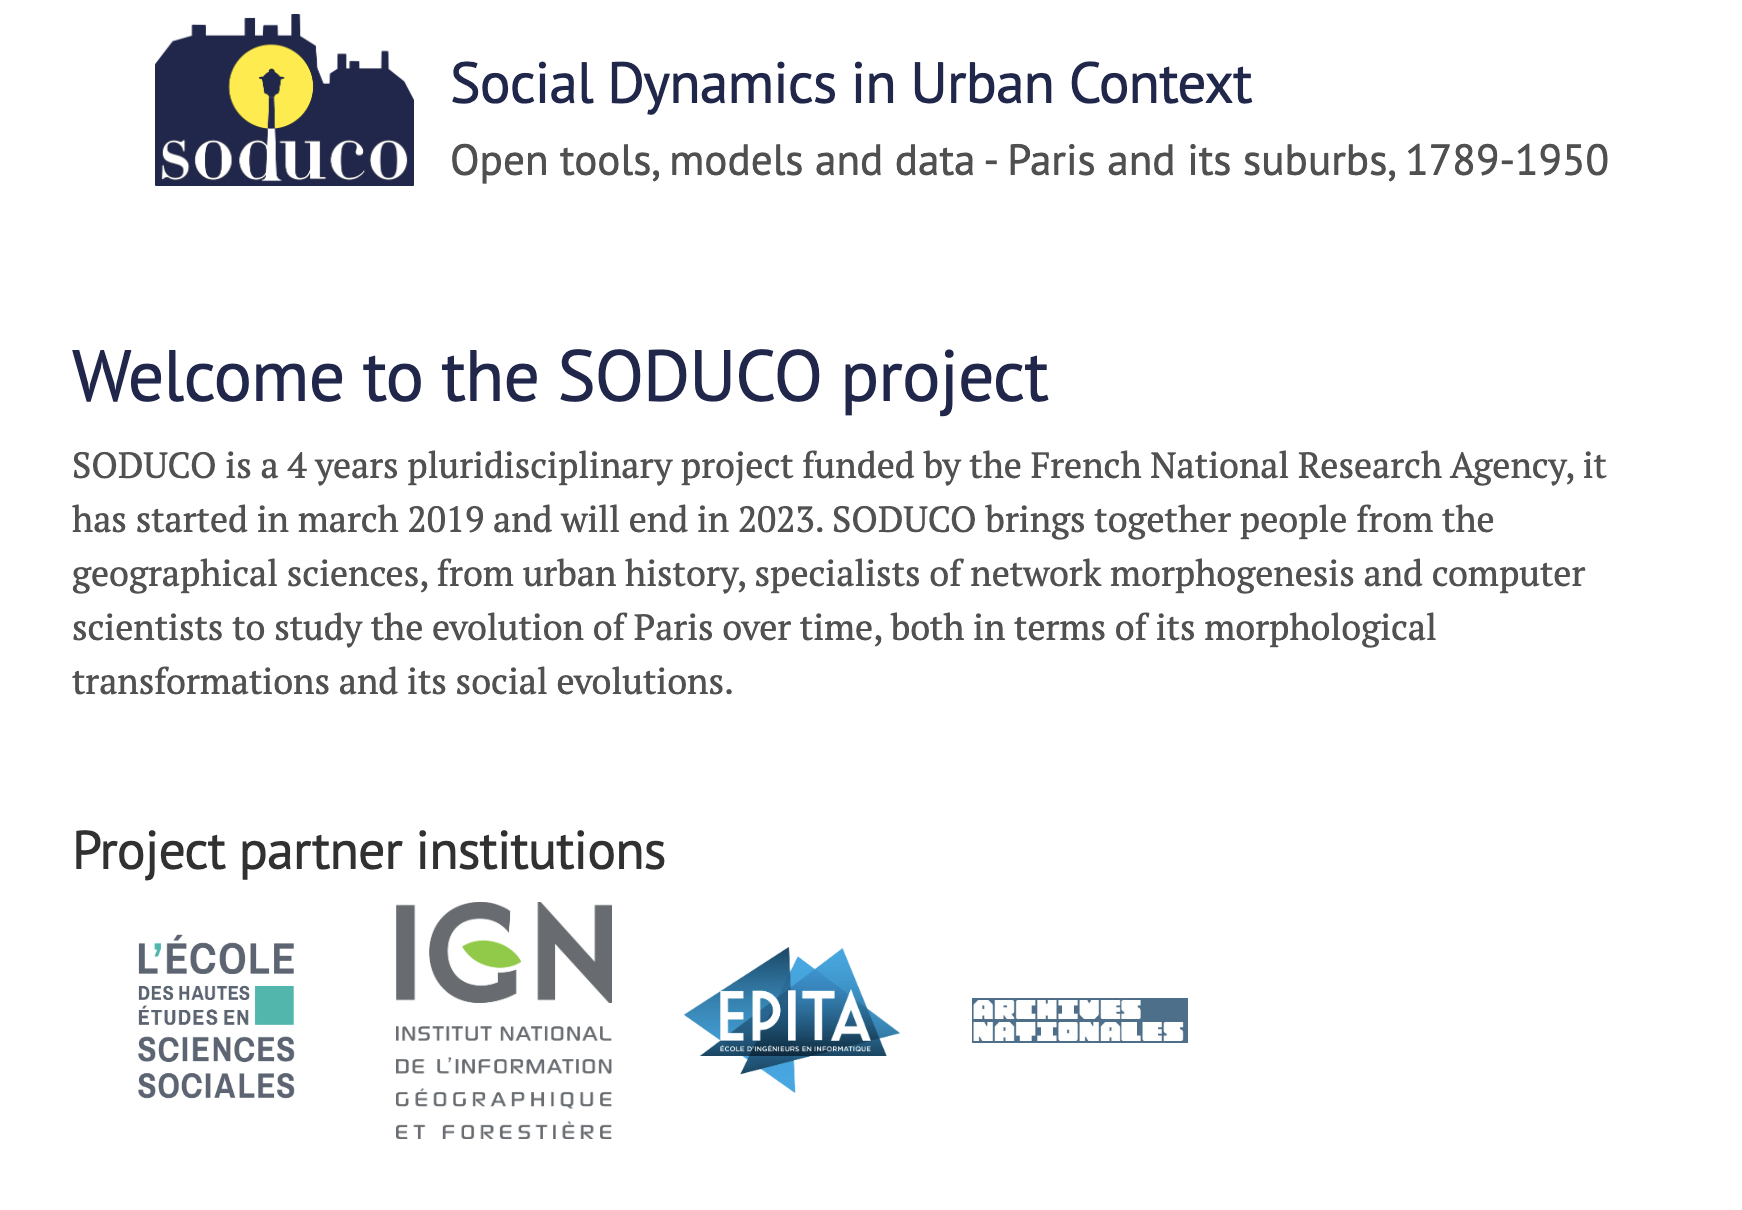
\includegraphics[height=0.85\textheight]{figures/soduco_presentation.png}
\end{center}t

\url{https://soduco.github.io/}

}


\sframe{Structure of the SODUCO project}{

\centering

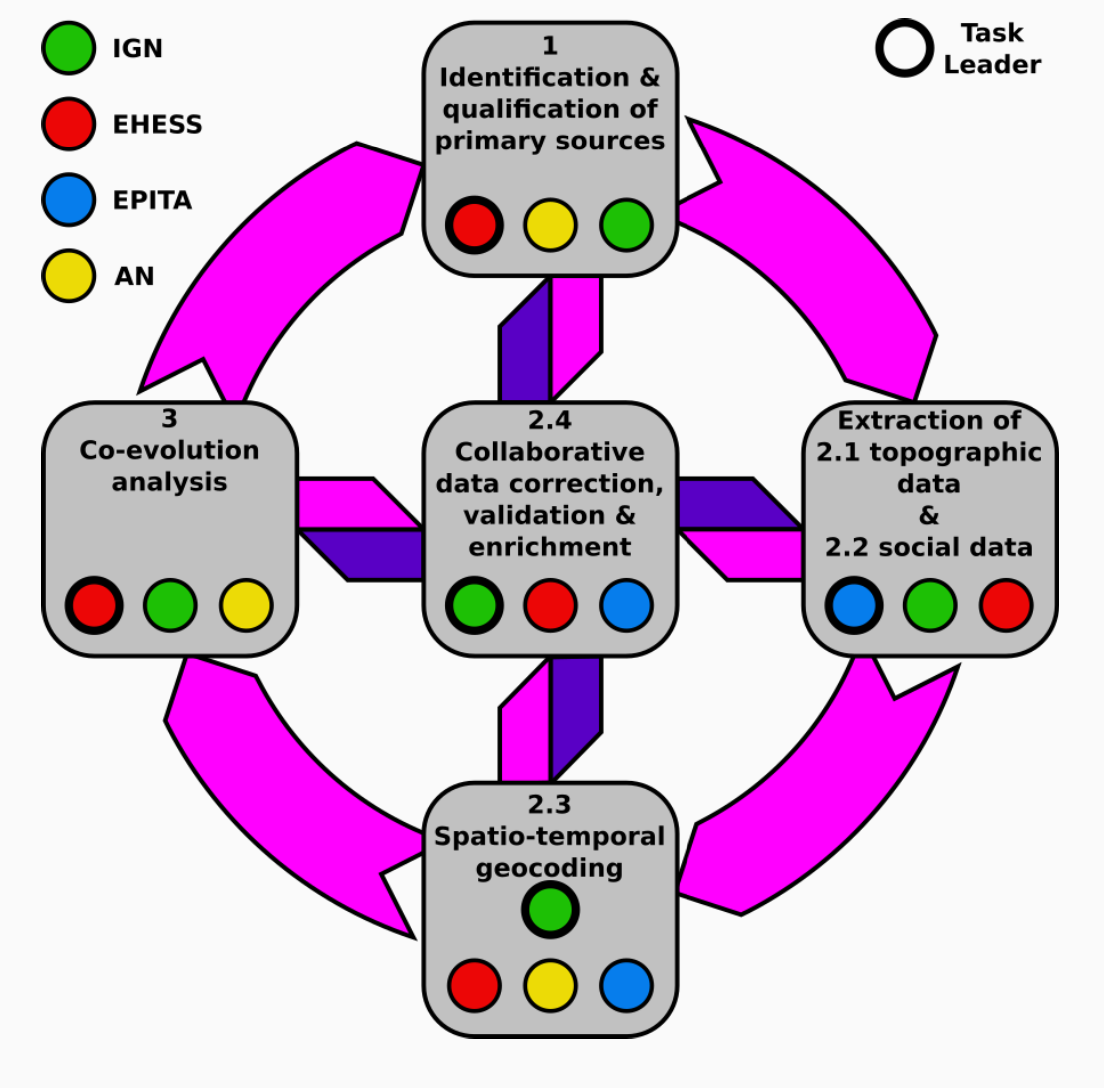
\includegraphics[height=0.9\textheight]{figures/soduco_structure.png}

}

\sframe{Project research objectives}{

% from slide kickoff
% 1. Identification et qualification des sources pertinentes Catalogue de sources primaires
%Qualification des sources et construction de méta-données
%Publication en ligne en (linked) Open Data Modélisation des imperfections associées
%2.1 et 2.2 Numérisation des sources
%Thèse avec EPITA sur l’extraction semi-automatique du contenu
%2.3 Géocodage des adresses
%2.4 Validation, correction et enrichissement collaboratifs 3. Analyse des co-évolutions
%Cartographie et géovisualisation des données et dynamiques associées
%Plateforme ouverte collaborative permettant la traçabilité des processus et des données 2 ans d’Ingénieur de recherche


\textbf{WP 1: Identification and qualification of relevant sources}

\medskip

$\rightarrow$ Catalog of primary sources; qualification of sources and metadata construction; online publication as Linked Open Data; modeling of uncertainties.

\bigskip

\textbf{WP 2: Digitalisation of sources}

\medskip

$\rightarrow$ Extraction of topographic data (2.1); extraction of socio-economic data (2.2); spatio-temporal geocoding (2.3); collaborative data correction, validation and enrichment (2.4).

\bigskip

\textbf{WP 3: Co-evolution analysis}

\medskip

$\rightarrow$ geovisualisation of data and associated dynamics.

\bigskip

\textbf{Tools: } collaborative open platform to ensure reproducibility and traceability of data and processes.



}

\sframe{Verniquet atlas accuracy}{

% other work packages?
% one slide on Verniquet georef - uncertainty: cool!

% critically analyse the Verniquet Atlas and especially its planimetric accuracy. We want to assess its potential for use as a historical cartographic reference resource.
% measurements and calculations provided with an accuracy of one tenth of a toise

% to understand the processes used by Edme Verniquet and his engineers to draw up the map, to check the measurements and calculations made and, if necessary, to correct their errors,
%to assess whether this map has a planimetric accuracy that is good enough for it to serve as a primary source to create a geohistorical reference dataset on the city of Paris at the end of the 18th century.
% One of the results of the Verniquet workshop is the reconstitution of the parameters of the projected coordinate reference system defined and used by Edme Verniquet to draw up his map of Paris. This reference coordinate system was reused throughout the 19th century in many other maps of Paris.

% https://github.com/soduco/Atlas-de-Verniquet

\begin{columns}
	\begin{column}{0.6\textwidth}
		\centering
		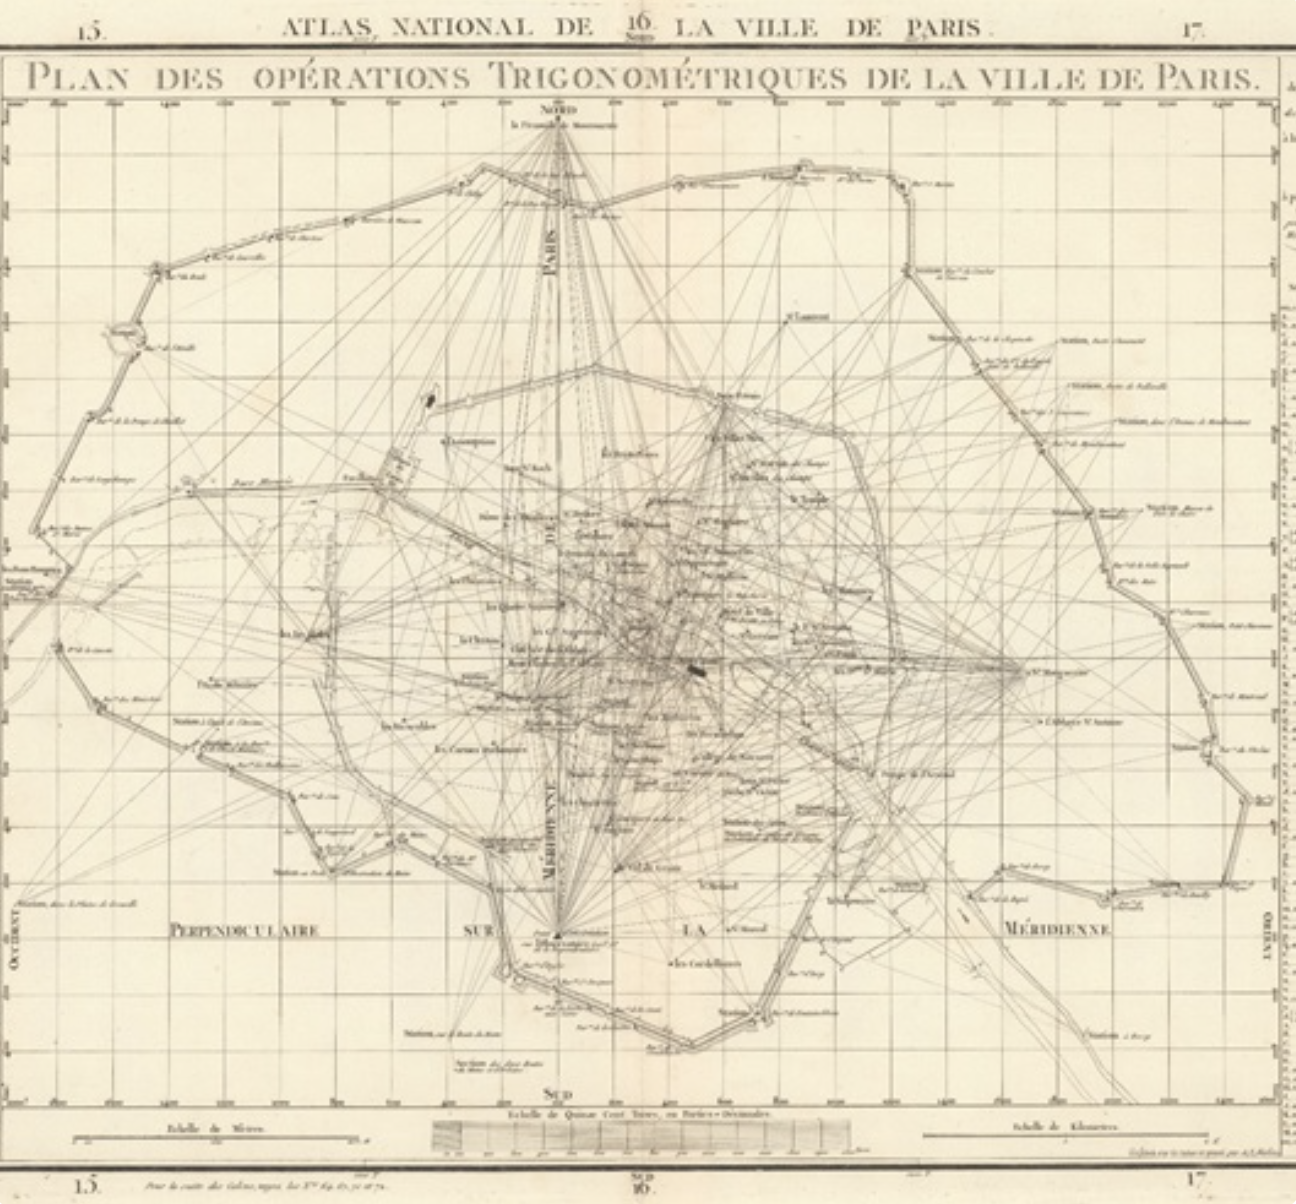
\includegraphics[width=\linewidth]{figures/verniquet.png}
	\end{column}
	\begin{column}{0.4\textwidth}
		\textit{Fieldwork survey with modern instruments to verify the planimetric accuracy of Verniquet atlas (claimed at 1/10 of a toise $\simeq$ 19cm)}
		
		\bigskip
		
		$\rightarrow$ Claimed uncertainties were correct
		
		\bigskip
		
		$\rightarrow$ CRS parameters for the historical coordinate system (reused as reference in many historical plans)
	\end{column}
\end{columns}


}

\sframe{Vectorisation of historical maps}{

% examples yizi thesis?

\begin{center}
	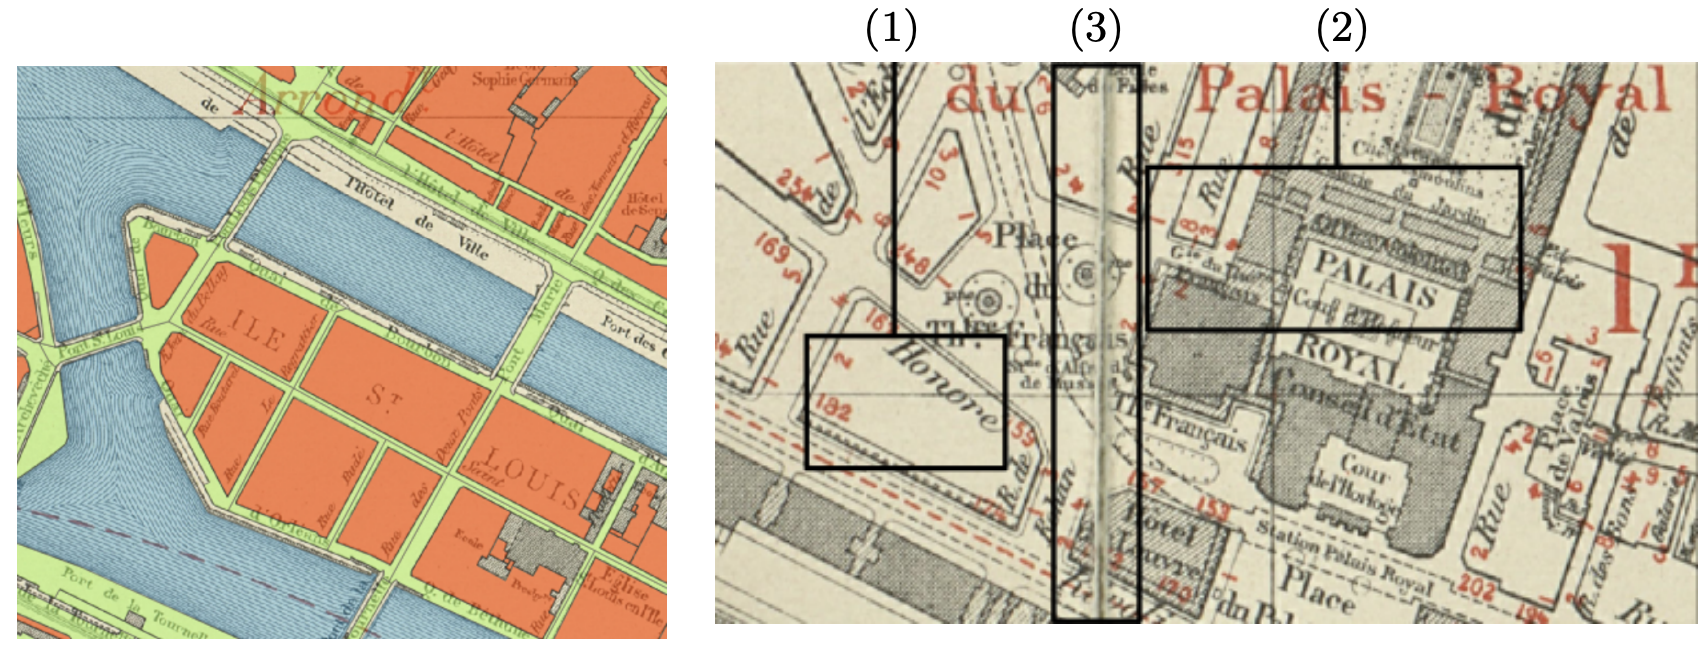
\includegraphics[width=\textwidth]{figures/vectorisation_issues.png}
	
	%\hrule
	
	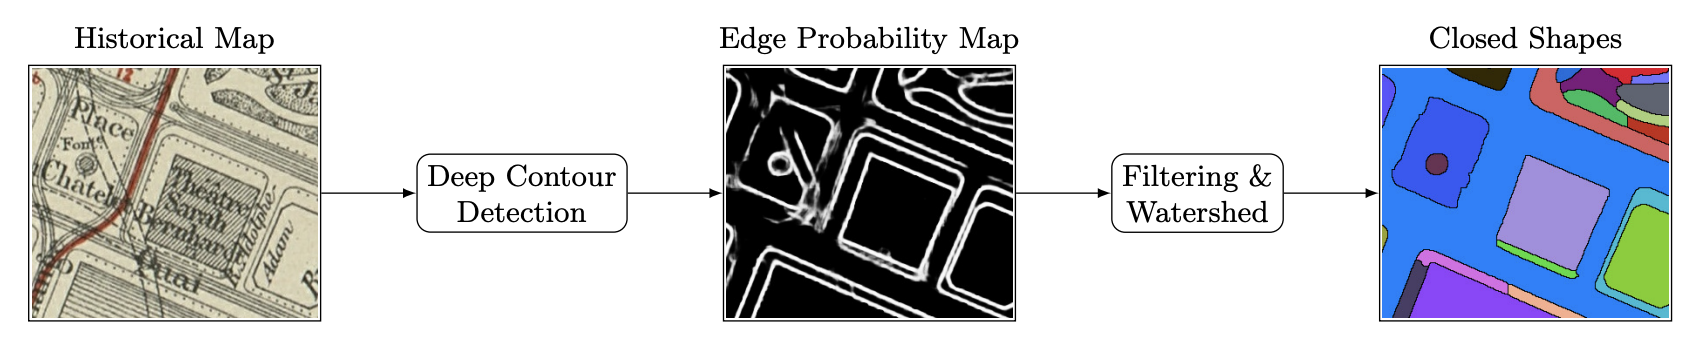
\includegraphics[width=\textwidth]{figures/vectorisation_workflow.png}
\end{center}

\footnotesize

\vspace{-0.5cm}

PhD thesis by Yizi Chen soon finished: vectorisation combining deep learning and mathemaatical morphology \cite{chen2021vectorization} \cite{chen2021combining}

}


\sframe{Quantification of intra-urban co-evolutionary dynamics}{

% this contribution research question / context 

%Urban systems are highly complex, what poses issues to ensure their resilience and sustainability and plan future cities [1]. One aspect of this complexity is their multidimen- sionality, even within subsystems such as the intra-urban location of economic activities. Indeed, different types of activities have specific location processes, yielding various patterns for their accessibility for example [2]. Understand- ing past dynamics of such social processes is crucial to build better urban models, theories and in practical terms insights for sustainable planning [3].


% [1] Michael Batty. Inventing future cities. MIT press, 2018.
%[2] Antonio Paez. Network accessibility and the spatial distri- bution of economic activity in eastern asia. Urban Studies, 41(11):2211–2230, 2004.
%[3] Celine Rozenblat, Denise Pumain, and Elkin Velasquez. In- ternational and transnational perspectives on urban systems. Springer, 2018.

$\rightarrow$ Multi-dimensionality of urban systems is one aspect of their complexity, strongly present in the co-evolution of economic activities locations.

\medskip

$\rightarrow$ Understanding past processes better inform urban theories and models for future sustainable planning.


\bigskip

\textbf{Research objective of this contribution (partly WP3): }

\medskip

\textit{Use geo-historical data to quantify the co-evolution of economic activities in Paris during the 19th century; methodological aspects on the issues linked to the exploitation of such data.}

}


\sframe{Urban systems and geo-historical data}{

% While recent and current urban dynamics are more and more easily tracked and quantified through the emergence of large urban data [4], historical dynamics on long time scales or on timeframes in a distant past are difficult to quantify due to the sparsity and heterogeneity of geo-historical data. At the macroscopic scale of urban systems, major transitions of past settlements systems have been modeled from an in- terdisciplinary perspective [5], and simulation models cap- turing various dimensions of systems of cities have been de- veloped [6]. At the mesoscopic and microsocpic intra-urban scales, several issues are encountered when trying to build consistent dataset, such as geocoding [7] or vectorisation to reconstruct the dynamics of road networks [8].

%[4] Jens Kandt and Michael Batty. Smart cities, big data and ur- ban policy: Towards urban analytics for the long run. Cities, 109:102992, 2021.
%[5] Lena Sanders. Peupler la terre: De la pre ́histoire a` l’e`re des me ́tropoles. Presses universitaires Franc ̧ois-Rabelais, 2018.
%[6] Denise Pumain and Romain Reuillon. Urban dynamics and simulation models. Springer, 2017.
%[7] Remi Cura, Bertrand Dumenieu, Nathalie Abadie, Benoit Costes, Julien Perret, and Maurizio Gribaudi. Historical col- laborative geocoding. ISPRS International Journal of Geo- Information, 7(7):262, 2018.
%[8] Hanae El Gouj, Christian Rincon-Acosta, and Claire Lagesse. Urban morphogenesis analysis based on geohistorical road data. Applied Network Science, 7(1):1–26, 2022.

$\rightarrow$ Contemporary intra-urban dynamics are better and better characterised through the emergence of urban data and urban analytics \cite{kandt2021smart}; more difficult with past dynamics.

\bigskip

$\rightarrow$ Interdisciplinary approaches to the modeling of settlement systems transitions: qualitative or very sparse data, stylised models (Transmondyn project) \cite{sanders2018peupler}

\bigskip

$\rightarrow$ Stylised models for systems of cities on long time scales \cite{pumain2017urban}

\bigskip

$\rightarrow$ Difficulty to build geo-historical data: geocoding \cite{cura2018historical}, vectorisation \cite{el2022urban}

}


\section{Data}

\sframe{Data extraction}{

% This contribution builds on data produced by the Soduco research project [9] to investigate co-evolutionary dynamics in the location of economic activities. More precisely, we focus on the case of Paris in the middle of the 19th cen- tury. Using public domain scans for main economic activ- ity repertoires (“Didot-Bottin”), an other work package of the project focused on building geo-referenced data contain- ing activities of various professionals, using Optical Char- acter Recognition techniques. We work on a sample of this data currently available, spanning 4 years between 1841 and 1844.

% -> example of Didot?

%[9] Social dynamics in urban context. Open tools, models and data - Paris and its suburbs, 1789-1950. https://soduco.github.io/.


\begin{columns}
	\begin{column}{0.6\textwidth}
		\centering
		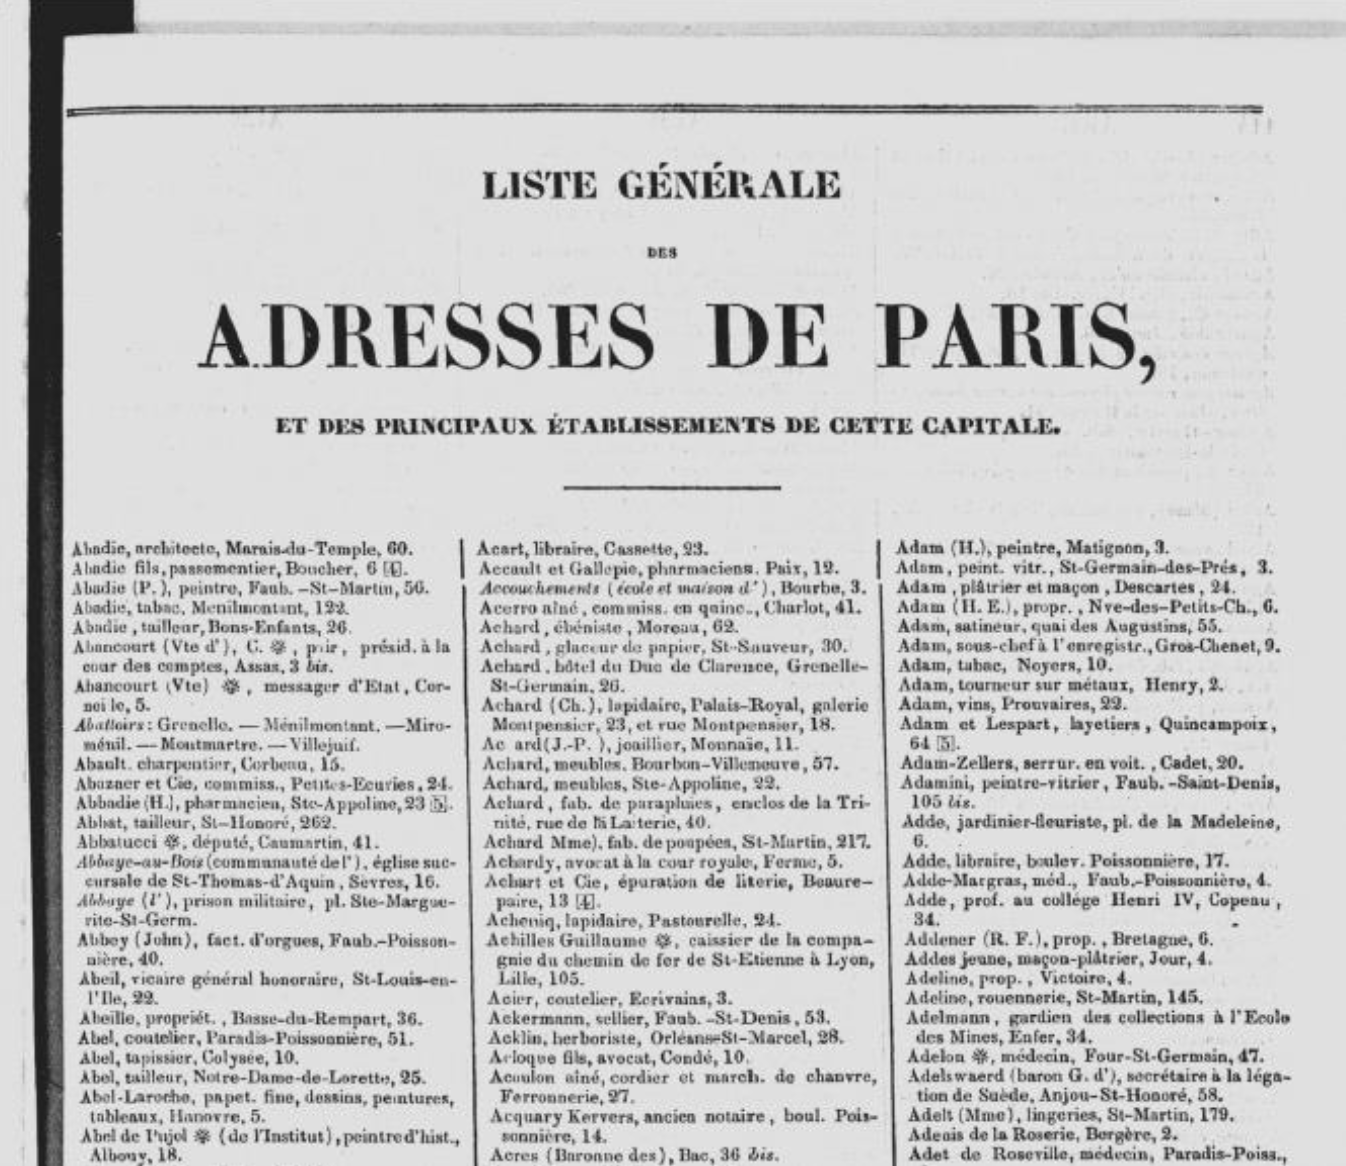
\includegraphics[width=\linewidth]{figures/didot.png}
	\end{column}
	\begin{column}{0.4\textwidth}
		
	\end{column}
\end{columns}




}


\sframe{Data pre-processing}{

% Starting from an initial dataset of 415,976 entries, we keep the ones with correct geographical coordinates (33%), and apply natural language processing (stemming and stop-word removal) to raw strings describing activities. From there, we focus on the stems with more than 100 occurences (578 stems), and code manually a broad category of economic activity for each (obtaining the coarse grain classification within: food, craftsmanship, art and literature, health, law and governance, service, teaching). We end at this stage with 36,072 entries with identified coordinates and broad ac- tivity. Source code and results are openly available on the git repository of this work at https://github.com/ JusteRaimbault/HistoricalData.




}


% includes "Methods"
\section{Results}

\sframe{Location of activities}{

% maps - to be redone !
% stored processed data? see other ordi tonight

}


\sframe{Definition and characterisation of co-evolution}{

% To study co-evolutionary dynamics, we use the defini- tion and characterisation method proposed by [10], which is based on weak Granger causality: two urban attributes will be co-evolving if they statistically exhibit a circualar causal relationship in this context.
% -> diagram soutenance? -> slides AG soduco

%[10] Juste Raimbault. Characterising and modeling the co- evolution of transportation networks and territories. arXiv preprint arXiv:2110.15950, 2021.



}


\sframe{Application to this dataset}{

% Aggregating spatially on raster cells (10x10 grid for the whole Paris), we thus com- pute lagged correlations between the variations of activity counts between successive dates for each cell, for each pair of activity. 

}


\sframe{Results: co-evolution}{

%We find several significant correlations (using Fisher confidence intervals), mostly negative for lagged cor- relations. This corresponds to a dynamic of sustitution of activities, with clusters rapidly replaced. Food and health are positively correlated and in co-evolution, while the other significantly co-evolving couple of activities is health and art but in a negative manner: in some districts medical pro- fessions replace artists and the contrary in others.

}

\sframe{Simultaneous correlations}{

%  We also consider simultaneous correlations, and find for example that food and craftsmanship have joint dynamics in the last time interval, but not during the first considered. 

}

\section{Discussion}

\sframe{Discussion}{

% Altogether, these results first confirm the existence of a co-evolution be- tween some activities, unveil a precise characterisation of intra-urban socio-economic dynamics, and open the path to- wards more advanced thematic interpretations within an in- terdisciplinary context, such as with historians.
% Current and future work also include (i) the extension of this study on longer time spans; (ii) the combination of Granger causality with geographically weighted regression, to optimise spatial neighbourhood considered in regressions [11], and (iii) the benchmark of methods to characterise co- evolution (including e.g. instrumental variables or causal machine learning methods) on this particular dataset.

%[11] Chris Brunsdon, Stewart Fotheringham, and Martin Charlton. Geographically weighted regression. Journal of the Royal Sta- tistical Society: Series D (The Statistician), 47(3):431–443, 1998.

}




\sframe{Conclusion}{

$\rightarrow$

\medskip

$\rightarrow$


\bigskip
\bigskip
\bigskip

\textbf{Soduco repository: }\\
\url{}

\bigskip

\textbf{Models and results open at }

\url{https://github.com/JusteRaimbault/HistoricalData}

}









%%%%%%%%%%%%%%%%%%%%%
\begin{frame}[allowframebreaks]
\frametitle{References}
\bibliographystyle{apalike}
\bibliography{biblio}
\end{frame}
%%%%%%%%%%%%%%%%%%%%%%%%%%%%





\end{document}













